\chapter{\IfLanguageName{dutch}{Stand van zaken}{State of the art}}
\label{ch:stand-van-zaken}

% Tip: Begin elk hoofdstuk met een paragraaf inleiding die beschrijft hoe
% dit hoofdstuk past binnen het geheel van de bachelorproef. Geef in het
% bijzonder aan wat de link is met het vorige en volgende hoofdstuk.
Bedrijven zijn constant op zoek naar betere en snellere resultaten. In het software development circuit is het vandaag soms nog lang wachten voor een wijziging effectief doorgevoerd wordt. Men levert nog vaak software op aan het einde van de sprint, wat soms voor problemen zorgt als men veel code tegelijk aflevert. Met een nieuwe software development methode - Continuous Integration en Continuous Delivery genaamd - wil men deze problemen zoveel mogelijk vermijden. Men spreekt vaak van een CI/CD pipeline als men het heeft over Continuous Integration en Continuous Delivery, maar er is nog een derde speler dat men kan invoeren: Continuous Deployment. Samen vormen zij de 3 musketiers om software projecten een grotere slaagkans te geven.
Om een duidelijker beeld te scheppen van een CI/CD pipeline zal dit hoofdstuk eerst uitleg verschaffen over DevOps, Continuous Integration, Continuous Delivery en Continuous Deployment. Daarna wordt er kort in detail gegaan hoe het bedrijf Amista eruit ziet en met welke tools ze werken. Tot slot wordt er uitgelegd hoe de grote structuur van een CI/CD pipeline eruit ziet.

% Pas na deze inleidende paragraaf komt de eerste sectiehoofding.
\section{DevOps}
\label{sec:devops}
    DevOps is een samentrekking van development en operations en is een welbekend begrip binnen de informatica wereld. Het heeft als doel om de 'state of mind' binnen een bedrijf te veranderen zodat alle lagen/departementen vlotter samenwerken. Het is een praktische 'gids' dat bedrijven kunnen gebruiken om de communicatie tussen developers en systeembeheerders beter te maken. Deze twee verschillende lagen in een bedrijf willen namelijk hetzelfde: zo snel mogelijk kwaliteitsvolle software opleveren. DevOps is gebaseerd op Agile development, maar gaat verder dan dat. Het gaat dieper in op automatisatie, integratie, samenwerking en communicatie. 
    Continuous Integration, Delivery en Deployment zijn kenmerkend voor DevOps, omdat het mee inzet op snellere oplevering van kwaliteitsvolle software. ~\autocite{Riti2018}
    
    % Hier zeker Patrick Debois vernoemen en vermelden waarom DevOps is opgericht: omdat ze in 2008 veel te maken hadden met falende projecten vanwege slechte communicatie.

\section{Continuous Integration}
\label{sec:continuous-integration}
    Dit is een eerste stap in de pipeline waarbij de geschreven code wordt gecommit naar een 'repository management server'. Hierdoor wordt de 'source code' automatisch opnieuw opgebouwd en slaagt voor de testen die automatisch zijn opgestart. De focus bij deze stap ligt bij de teamleden ~\autocite{Fowler2006}, van hen wordt verwacht dat ze -op een regelmatige basis- hun code pushen (integreren met de master applicatie). Een goede samenwerking tussen de verschillende leden van het development team is broodnodig om tot het gewenste eindresultaat te bekomen.
    Het doel van een Continuous Integration is om de integratie feilloos te laten verlopen wanneer men software ontwikkelt en geen functionaliteiten verliezen na een merge ~\autocite{Riti2018}.
    \newline
    Bovenstaande uitleg is makkelijker te begrijpen aan de hand van een voorbeeld. Op Figuur \ref{img-ci-example} is een grafische voorstelling van dit voorbeeld terug te vinden.
    De developer commit code naar de repository die te vinden is op het source-control systeem. De Continuous Integration server krijgt het bericht dat er code is toegevoegd, haalt de laatst toegevoegde code op en laat de testen runnen. Wanneer alle testen slagen zal de CI server de code compilen en feedback bezorgen aan de developer. In dit voorbeeld maakt men gebruik van een externe mail server om die feedback te verzenden.
    Deze stappen gebeuren elke keer er code naar de repository gestuurd wordt.

    \begin{figure}	
        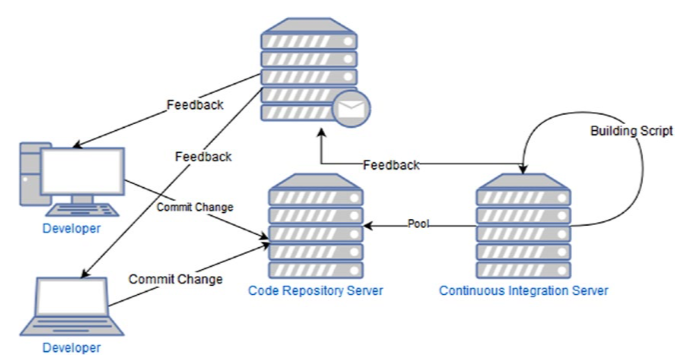
\includegraphics{ci-example}
        \caption{Voorbeeld van een Continuous Integration set-up ~\autocite{Riti2018}} \label{img-ci-example}
    \end{figure}

\section{Continuous Delivery}
\label{sec:continuous-delivery}
    Eens het team met succes de Continuous Integration toepast kan men overschakelen naar de volgende stap: Continuous Delivery.
    Het is een manier dat ervoor zorgt dat de code die van de Continuous Integration stap komt gebuild wordt en voorbereidt wordt voor een release.
    Er is echter wel nog een menselijk hand nodig om de build van deze stap te deployen en voor de buitenwereld beschikbaar stellen ~\autocite{Fowler2013}.
    

\section{Continuous Deployment}
\label{sec:continuous-deployment}
    De gelijkenis met Continuous Deployment is treffend, maar er is wel degelijk een verschil.
    Hier gaat men automatisch de veranderde code naar productie brengen. De veranderingen gaan door de volledige pipeline en eens ze slagen voor alle testen wordt - zonder menselijke interactie - de code naar productie gebracht ~\autocite{Claps2015}.
    Dit wordt soms ook wel de 'train to production' genoemd, omdat elke code dat gepushed wordt naar de source-control automatisch tot bij de klant geraakt.

\section{Amista}
\label{sec:amista}
    Amista is een groeiend bedrijf binnen IT consultancy. Het is een dochterbedrijf van Boutique dat zich toespitst op SAP. Sinds hun vijfjarig bestaan werken er al 60 personen voor Amista. Ze hebben Infrabel, Alcopa, Danone, AG Real Estate en nog anderen tot hun cliënteel, zoals op hun site staat te lezen ~\autocite{Amista2018}.
    Ze zijn in twee landen actief, Frankrijk en België, maar werken ook samen met mensen uit India.
    Amista heeft zich verdiept in de Sales, Marketing en Service Management takken van bedrijven. Ze helpen hun klanten ook op gebied van Innovation, Integration, HCM Services(implementeren van succesfactoren binnen de HR afdeling) en Digital Learning.
    De missie van Amista is om samen met hun klanten innovatieve en kwalitatieve oplossingen aan te bieden met behulp van het vollediga gamma dat SAP te bieden heeft.
    Omdat Amista graag wil innoveren en de wensen van hun klanten zo goed mogelijk probeert uit te voeren, zijn ze aan het kijken om te investeren in een CI/CD pipeline. Er is nog niet veel informatie te vinden hoe men een CI/CD pipeline kan integreren in SAP Cloud Platform, maar Amista wil de uitdaging aangaan. 

\section{SAP}
\label{sec:sap}
    SAP is een Duitse onderneming opgericht in 1972 dat softwareoplossingen aanbiedt voor grote ondernemingen. Met meer dan 413.000 klanten verspreid over 180 landen mag SAP zich marktleider noemen op gebied van bedrijfssoftware.
    SAP heeft zicht gespecialiseerd in ERP, Enterprise Resource Planning software dat alle processen van het bedrijf automatiseert ~\autocite{SAPERP2019}. Een ERP systeem beheert meerdere functies en bedrijfsprocessen van 1 bedrijf op basis van een gezamelijke database. Het heeft als doel de gegevens van de organisatie optimaal te gebruiken in de gehele organisatie en een betere beheersing van de bedrijfsprocessen voorzien.
    De oplossingen dat SAP aanbiedt is vooral bedoeld voor de grotere bedrijven. Ze bieden software aan voor elke mogelijke industrie die er vandaag de dag bestaat. Momenteel zijn ze gespecialiseerd in cloud business software.

\section{SAPUI5 webapplicatie volgens Amista}
\label{sec:sapui5-sap-hana}
    Amista heeft enkele klanten waar ze SAPUI5 webapplicaties voor moeten maken. Deze combineren ze met een SAP HANA database dat allemaal draait op SAP Cloud Platform. Omdat er nog niet veel informatie te vinden is over een CI/CD pipeline binnen bovenstaande toepassingen, wil Amista heel graag een gepersonaliseerde handleiding om zo een pipeline op te stellen.
     
    \paragraph{SAP Cloud Platform}
        SAP Cloud Platform is een platform as a service (PaaS), dat aangeboden wordt door SAP. het is een online platform dat - door hardware en software samen te brengen - applicaties overal toegankelijk maakt en samenbrengt tot 1 platform online ~\autocite{SAPSE2018}.
        SAP Cloud Platform wordt zowel voor development als deployment gebruikt, maar reikt ook de hand aan verschillende technologieën: Internet of Things, big data, Artificiële Intelligentie enzovoort. Het is een platform dat zowel on-premise - waarbij software enkel lokaal op een computer beschikbaar is - als cloud technologieën samen kan brengen. Je kan er de technologieën ook uitbreiden en zelf ontwikkelen. Het haalt zijn kracht uit de perfecte integratie met andere SAP software die je ook nog eens kan uitbreiden.
    
    \paragraph{SAPUI5}
        SAPUI5 is een framework dat uitgevonden is door SAP en bevat verschillende libraries die bovenop JavaScript gebouwd zijn. Men kan via het SAP Cloud Platform front-end applicaties maken en deployen die geschreven zijn in SAPUI5. Het is een framework dat bedoeld is om HTML5 applicaties te bouwen die bijna automatisch responsive zijn zonder veel bijkomende code toe te voegen.
        Het is bedoeld om dezelfde lay-out en hetzelfde gebruik voor de eindklant te garanderen. Het biedt aan de developers een resem aan UI controls aan zodat er een consistenter en beter UX design gehanteerd wordt.~\autocite{SAPSEa} 
    
    \paragraph{SAP HANA}
        In-Memory Data Platform staat er er als titel op de site van SAP te lezen. Het is een platform dat gebruik maakt van het RAM geheugen van de computer, wat enorme snelheden met zich meebrengt, maar ook een enorm kostenplaatje. Dit even terzijde wordt SAP Hana aangeprezen als een platform  om ingewikkelde, real-time analytische berekeningen uit te voeren op data.
        Het is een relationeel database management systeem (RDMBMS) dat geïntegreerd kan worden in SAP Cloud Platform, waarbij het mogelijk is om zowel on-premise als in de cloud te werken, of een combinatie van beiden. 

\section{Tools voor een CI/CD pipeline}
\label{sec:tools-voor-pipeline}
    Er bestaan verschillende repository management services die een source control systeem hebben. GitHub, GitLab en Bitbucket zijn enkele voorbeelden uit het rijtje.
    Build schedulers zorgen ervoor dat de procedures worden samengesteld en dat de builds worden getriggerd. Voorbeelden hiervan zijn: Jenkins, Travis CI, GitLab-CI en Bamboo. Sonatype Nexus en Archiva zijn dan weer voorbeelden van tools die gebruikt worden als artifact repository manager, deze houden bij wijze van spreken de code bij die klaar is om te deployen. 
    
    \paragraph{Source Control System}
    Dit systeem houdt alle veranderingen bij aan de code en zal de veranderingen ook beheren zodat ze niet overlappen. Het laat toe dat meerdere developers tegelijk aan - soms dezelfde - code werken. Een source control systeem houdt dan de veranderingen bij wat elke developer gedaan heeft. Best practice is er maar 1 versie van de software die stabiel is, meestal master genoemd. Een gangbare praktijk binnen dit systeem is het maken van branches. Hier wordt een kopie gemaakt van de stabiele master, waardoor men wat kan knoeien in de branch zonder de master te beschadigen. Als men overtuigd is van de kwaliteiten dat men op een branch gemaakt heeft kan men de branch 'mergen' in de master. Deze techniek wordt ook wel 'revision control' of 'version control' genoemd ~\autocite{Skelton2014} en ~\autocite{Riti2018}.
    Voorbeelden van zo een source control system zijn Git, CVS (Concurrent Version System), Subversion en Mercurial.
    
    \paragraph{Repository Management Services}
    Wordt ook wel Code Repository Server genoemd. Hier wordt de software van het source control system opgeslagen. Dit kan op een interne server opgeslagen worden, of op een externe die door bedrijven aangeboden wordt. Dit maakt het makkelijker voor developers om samen te werken en dezelfde bron te gebruiken en is nodig om een goede Continuous Integration aan te bieden.
    
    \paragraph{Build Scheduler of Continuous Integration Server}
    Dit zorgt ervoor dat - telkens wanneer er code gecommit wordt - de pipeline wordt uitgevoerd. De taken van de build scheduler zijn: 
    \begin{itemize}
        \item Code ophalen van de Repository Server en deze samenvoegen met de oude code
        \item De testen uitvoeren
        \item Het builden van de software
        \item Feedback geven aan de developer over voorgaande stappen
    \end{itemize}
    Deze taken kunnen ook door een script volbracht worden, maar het is belangrijk dat deze taken automatisch gebeuren telkens er code gecommit wordt naar de repository manager ~\autocite{Riti2018}.
    
    \paragraph{Artifact Repository Manager}
    Als laatste zijn de Artifact Repository Managers aan de beurt. Deze repository manager houdt alles wat nodig is om de applicatie te deployen bij zoals
    \begin{itemize}
        \item packaged application code
        \item application assets
        \item infrastructure code
        \item virtual machine images
        \item configuration data
    \end{itemize}
    Deze tool houdt alle geschiedenis bij van de bovenstaande files. Zoals eerder vermeld kan men vanaf hier de software (automatisch) deployen. Dit is de allerlaatste fase in de CI/CD pipeline ~\autocite{Skelton2014}.
    
% \lipsum[7-20]
